\documentclass{article}%
\usepackage[T1]{fontenc}%
\usepackage[utf8]{inputenc}%
\usepackage{lmodern}%
\usepackage{textcomp}%
\usepackage{lastpage}%
\usepackage{authblk}%
\usepackage{graphicx}%
%
\title{Katanin Localization Requires Triplet Microtubules in Chlamydomonas reinhardtii}%
\author{Bradley Lewis}%
\affil{Oncology Research, Pfizer Worldwide Research and Development, San Diego, California, United States of America}%
\date{01{-}01{-}2009}%
%
\begin{document}%
\normalsize%
\maketitle%
\section{Abstract}%
\label{sec:Abstract}%
In a new study, scientists report the potential for treatment of diabetic nephropathy in mice.\newline%
The paper has been published in the November issue of Cell Reports.\newline%
The study used a mouse model of the immune system associated with diabetic nephropathy.\newline%
Unlike many other treatments that seek to slow down the level of immune responses, researchers found the treatments produced so{-}called hyperkalemia  a significant increase in the function of the immune system in mice with the condition.\newline%
Published results showed that the treatment was very effective and helped control disease progression.\newline%
Researchers say this findings could help address two key issues that plague diabetics  what needs to be done about nerve growth factors and how to stem the growth of new tumors in diabetic nephropathy.

%
\subsection{Image Analysis}%
\label{subsec:ImageAnalysis}%


\begin{figure}[h!]%
\centering%
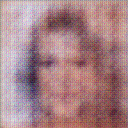
\includegraphics[width=150px]{500_fake_images/samples_5_231.png}%
\caption{A Close Up Of A Black And White Cat}%
\end{figure}

%
\end{document}